\chapter{Additional Figures}

\section{Repeater Backbone and Purification}
\label{app:figures}

This section collects illustrative figures supporting Chapter~\ref{chap:background} that are too detailed to place inline without interrupting its narrative: the elementary Bell-state measurement, a worked example of backbone selection across a full chain, and the circuit-level implementation of the three purification circuits.

\subsection{Bell-State Measurement}

Section~\ref{sec:bg:bellpairs} introduces the Bell-state measurement (\Gls{bsm}) as the elementary operation used to establish and extend entanglement links. Figure~\ref{fig:bsm} illustrates it in more detail than the main text.

\glsreset{bsm}
\begin{figure}[h]
    \centering
    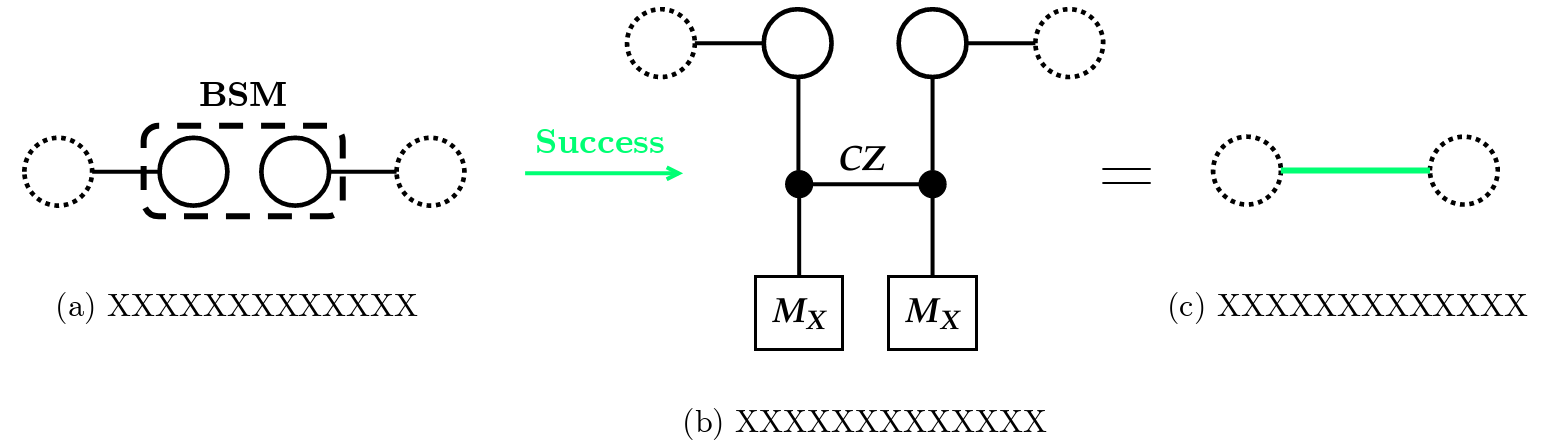
\includegraphics[width=\textwidth]{figures/background/BSM_combo.png}
    \caption{Entanglement swapping via a linear-optical \Gls{bsm}. \textbf{(a)} Two incoming photonic qubits from neighbouring resources interfere at a beamsplitter and are measured in the computational basis. Only two of the four Bell states are distinguishable, limiting the success probability to 50\% per attempt (Section~\ref{sec:bg:bellpairs}). \textbf{(b)} Graph-state representation of a successful \Gls{bsm}, equivalent to a $CZ$ gate followed by $X$-basis measurements ($M_X$) on the measured qubits. \textbf{(c)} The resulting edge (green) directly connects the two remaining qubits, establishing entanglement between the neighbouring resources.}
    \label{fig:bsm}
\end{figure}

\subsection{Backbone Selection Example}

Section~\ref{sec:bg:backbone} describes \emph{backbone selection}: at every \Gls{absa}, the first arm whose \Gls{bsm} succeeds is kept and every other arm at that hop is discarded, regardless of which arm that turns out to be. Figure~\ref{fig:app:backbone-selection} works through a concrete 3-hop chain to make this concrete: each \Gls{absa} independently keeps whichever of its arms first succeeds, and the surviving entanglement (bottom row) connects Alice to Bob only through the chain of kept arms, one hop at a time, regardless of which specific arm succeeded at each hop.

\begin{figure}[ht]
    \centering
    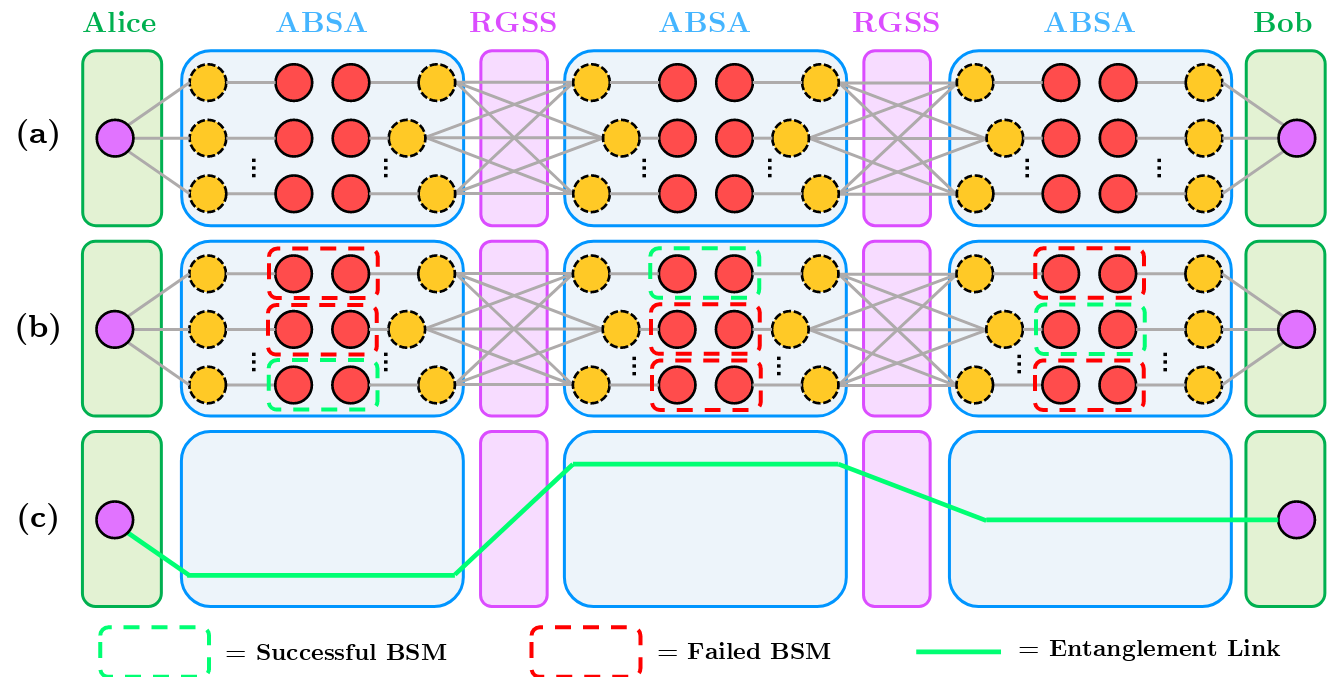
\includegraphics[width=\textwidth]{figures/background/ES_process.png}
    \caption{Backbone selection across a $N=3$-hop chain. \textbf{(a)} The network configuration before entanglement generation. Each \Gls{absa} initially holds outer/inner qubit pairs (red/yellow) for all provisioned arms connecting it to each of its two neighbouring stations. \textbf{(b)} At each \Gls{absa}, a \Gls{bsm} is attempted for every available arm. Multiple attempts may succeed, but once at least one successful \Gls{bsm} is obtained (green), one successful arm is selected and its corresponding inner qubits are retained, while the remaining arms are discarded. As this selection is performed independently at each \Gls{absa}, the retained arms need not correspond to the same arm index across the different hops. \textbf{(c)} The selected inner qubits form the backbone used to establish end-to-end entanglement. The resulting entanglement (green line) connects Alice to Bob through one retained arm at each hop, as described in Section~\ref{sec:bg:backbone}.}
    \label{fig:app:backbone-selection}
\end{figure}

\subsection{Purification Circuits}

Section~\ref{sec:bg:circuits} introduces the three purification circuits $\mathcal C_\mathrm{ZX}$, $\mathcal C_\mathrm{XZ}$, and $\mathcal C_\mathrm{YY}$ by the stabilizer each one measures. Figure~\ref{fig:app:circuits} below gives their circuit-level implementation.

% Circuit-level diagrams for the three purification circuits of
% Section~\ref{sec:bg:circuits}/\ref{sec:bg:purmath}. Each circuit acts on
% one retained and one measured qubit per party (Alice/Bob); the retained
% qubit survives as the purified output on success, the measured qubit is
% consumed by the local measurement whose outcome is compared between
% parties to determine success.

\begin{figure}[htbp]
    \centering

    \begin{subfigure}[t]{0.30\textwidth}
        \centering
        \begin{quantikz}[row sep=0.32cm, column sep=0.34cm]
            \lstick[2]{Alice} & \ctrl{1}  & \qw      & \qw      & \qw \\
                              & \targ{}   & \meter{} & \qw      & \qw \\
            \lstick[2]{Bob}   & \targ{}   & \qw      & \qw      & \qw \\
                              & \ctrl{-1} & \gate{H} & \meter{} & \qw
        \end{quantikz}
        \caption{$\mathcal C_\mathrm{ZX}$}
        \label{fig:app:circuit-zx}
    \end{subfigure}
    \hfill
    \begin{subfigure}[t]{0.30\textwidth}
        \centering
        \begin{quantikz}[row sep=0.32cm, column sep=0.34cm]
            \lstick[2]{Alice} & \targ{}   & \qw      & \qw      & \qw \\
                              & \ctrl{-1} & \gate{H} & \meter{} & \qw \\
            \lstick[2]{Bob}   & \ctrl{1}  & \qw      & \qw      & \qw \\
                              & \targ{}   & \meter{} & \qw      & \qw
        \end{quantikz}
        \caption{$\mathcal C_\mathrm{XZ}$}
        \label{fig:app:circuit-xz}
    \end{subfigure}
    \hfill
    \begin{subfigure}[t]{0.36\textwidth}
        \centering
        \begin{quantikz}[row sep=0.32cm, column sep=0.22cm]
            \lstick[2]{Alice} & \gate{H}         & \gate{S^\dagger} & \ctrl{1} & \gate{S} & \qw      & \qw \\
                              & \gate{H}         & \gate{S^\dagger} & \targ{}  & \gate{H} & \meter{} & \qw \\
            \lstick[2]{Bob}   & \gate{S^\dagger} & \ctrl{1}         & \gate{S} & \qw      & \qw      & \qw \\
                              & \gate{S^\dagger} & \targ{}          & \gate{H} & \meter{} & \qw      & \qw
        \end{quantikz}
        \caption{$\mathcal C_\mathrm{YY}$}
        \label{fig:app:circuit-yy}
    \end{subfigure}

    \caption{Circuit-level implementation of the three purification circuits introduced in Section~\ref{sec:bg:circuits}. Each circuit consumes two same-span resources, one held by Alice and one by Bob (top/bottom wire per party is the retained/measured qubit respectively), and produces one purified resource on the retained wires when the two parties' measurement outcomes agree. \textbf{(a)} $\mathcal C_\mathrm{ZX}$: Alice measures the $Z$-parity of her pair (\textsc{cnot} into her measured qubit, then measurement) while Bob measures the $X$-parity of his (\textsc{cnot} into his retained qubit, Hadamard, then measurement); success probability and output error vector in Eqs.~\eqref{eq:pzx} and~\eqref{eq:purzx}. \textbf{(b)} $\mathcal C_\mathrm{XZ}$: the same construction with Alice and Bob's local circuits exchanged, so Alice measures the $X$-parity and Bob the $Z$-parity (Eqs.~\eqref{eq:pxz}, \eqref{eq:purxz}). \textbf{(c)} $\mathcal C_\mathrm{YY}$: both parties apply a local $H$--$S^\dagger$ basis change before their \textsc{cnot}, so the compared parity is a joint $Y$-type stabilizer across all four qubits (Eqs.~\eqref{eq:pyy}, \eqref{eq:puryy}).}
    \label{fig:app:circuits}
\end{figure}

\clearpage

\section{Pseudocode and Concurrency Analysis}
\label{app:concurrency}

Section~\ref{sec:model:budget} defines the concurrency requirement $M(\Sigma)$ and its Sethi--Ullman recurrence~\cite{Sethi1970Generation}. This appendix gives the pseudocode implementing that recurrence as well as a complexity analysis.

The following pseudocode implements this recurrence. It assumes that the schedule is a binary tree and that each node exposes its children through $\texttt{children}(v)$.

\begin{algorithm}[ht]
\DontPrintSemicolon
\SetKwFunction{FRegReq}{RegisterRequirement}
\SetKwProg{Fn}{Function}{:}{}
\Fn{\FRegReq{$v$}}{
    \If{$v$ is \textup{\texttt{GenNode}}}{\Return $1$\;}
    \If{$v$ is \textup{\texttt{IdleNode}} or $v$ is \textup{\texttt{HeraldNode}}}{
        $c \gets \texttt{child}(v)$\;
        \Return \FRegReq{$c$}\;
    }
    $(c_1,c_2) \gets \texttt{children}(v)$\;
    $L \gets$ \FRegReq{$c_1$}\;
    $R \gets$ \FRegReq{$c_2$}\;
    \eIf{$L \neq R$}{\Return $\max(L,R)$\;}{\Return $L+1$\;}
}
\caption{Minimum concurrency requirement of a tree-shaped schedule}
\label{alg:concurrency}
\end{algorithm}

The procedure is evaluated recursively from the root, so every node is visited exactly once. Consequently, the computation takes $O(|T|)$ time and $O(h)$ auxiliary space for a tree of $|T|$ nodes and height $h$. The resulting value is thus the concurrency requirement $M(\Sigma)=\textsc{RegisterRequirement}(\mathrm{root}(T))$. The schedule satisfies the concurrency budget when $M(\Sigma)\leq M_{\max}$.